\chapter{Synthesis of Probabilistic Programs} \label{chap:synthesis_methods}

\section{Automated System Design}

The~dream of automating software development has been present since the~beginning of the~computer age. 
As early as 1945,~as part of an~ideal vision for an~automatic computing machine,~Alan Turing argued that the~process of compiling instruction tables would be fascinating,~free of errors and no effort,~as the~machine itself would perform all demanding operations.
What if we could tell the~computer what to do \,--\, or give it a~specification of what we want as users \,--\, and let it work to figure out how to do it? 
This is the~promise of program synthesis,~where after entering a~specification,~the~computer automatically generates a~program that satisfies that specification.

\paragraph{Deductive Synthesis.}
The~earliest examples of program synthesis used formal specifications to infer the~correct program automatically. 
The~aim is to take a~formal specification and search backwards for a~program that provably satisfies the~specification. 
Some of the~synthesisers in this area relied on the~successes of automated theorem provers,~which they used to compile proof of program accuracy. 
Others used a~comprehensive set of rewriting rules in an attempt to transform a~specification into an~equivalent program. 
This approach is similar to a~regular compiler transforming the~input program into an~output program using rewriting rules from specified grammar. 
However,~the~rewriting rules of the~synthesiser should be complete \,--\, the~synthesiser tries to find the optimal program \,--\, and should be able to transform the~specification into every equivalent program.
The~landmarks in this area are works based on super-optimisation~\cite{superoptimiser} and the Synthesis kernel~\cite{kernel}.

\paragraph{Syntax-Guided Synthesis.}
The~obstacle of deductive synthesis is that it requires both a~complete formal specification and a~complete axiomatisation of the program target language.
The~second wave of synthesis research focuses on the~\textit{syntax-driven} synthesis,~trying to relax these requirements. 
The~input to the \textit{syntax-guided} synthesis problem consists of a~semantic correctness specification for the~desired program given by a~logical formula and a~syntactic set of candidate programs.
This set is described by a~sketch~\cite{sketching} (program template) containing undefined locations described as yet unknown system properties or maybe intentionally omitted. 
Approaches of this second wave have recently come to the~fore,~and our approach is also based on them. 

\section{Related Work}

The~synthesis tasks for parametric probabilistic programs can be divided into the~following two categories.

\paragraph{Topology Synthesis.}
This synthesis task considers a~finite set of parameters that affect the~\textit{topology} of Markov chains.
Finding a~family member that satisfies given specifications is \textit{NP}-complete in the~parameters' number and can be naively solved by analysing all individual family members~\cite{onebyone}.
An~alternative approach models the~family of MCs by an~MDP and uses off-the-shelf algorithms for MDP model-checking~\cite{allinone}.
Tools such as \emph{QFLan}~\cite{qflan} and \emph{ProFeat}~\cite{profeat} implements these approaches to quantitatively analyse alternative designs of software product lines~\cite{sw-product-lines}.
These tools provide the~complete methods to solve synthesis tasks,~but they are limited strictly to small families,~so they do not scale.
Inductive techniques,~motivated from these basic approaches,~form on abstraction-refinement (\emph{AR}) over the MDP representation~\cite{cegar},~and counterexample guided inductive synthesis (\emph{CEGIS}) for MCs~\cite{cegis} have been proposed to achieve better scalability.
Experiments in previous papers~\cite{cegar,cegis} have shown that the~synthesis methods implemented in \emph{ProFeat} or \emph{QFLan} have evident deficits on the~benchmarks investigated also in this thesis.
This synthesis task is closely connected to controller synthesis for partially observed MDPs (POMPDs),~representing,~for instance,~a~famous Maze~\cite{maze} model for AI planning under uncertainty,~to which we will pay attention later.
Other techniques to solve the~controller synthesis for POMDPs also use neural network oracles to lead search~\cite{pomdp-2} and adaptive learning schemes based on imitation learning~\cite{POMDP3}.

\paragraph{Parameter Synthesis.}
It considers models with a~fixed topology but with uncertain parameters associated with transition probabilities (or rates).
It analyses how the~parameter values affect the~behaviour of Markov chains (or MDPs).
\textit{Parameter} synthesis problems targets finding parameter values for which the~parametric model (optimal) satisfies the~specification.
The~state-of-the-art probability model checkers \storm{}~\cite{STORM} and \prism{}~\cite{KNP11} provide approximate techniques for parameter synthesis that solve the~same parameters in various transitions independently.
We note that these model checkers and others with the~same focus are primarily determined to verify concrete MC and not to the~whole MCs family.
On the contrary,~exact techniques construct rational functions for symbolic reachability probabilities have been proposed in~\cite{DBLP:conf/ictac/Daws04} and further improved in~\cite{dehnert2015prophesy}.
% The~application of this synthesis task can be found, for instance,~in the~field of model repair problems~\cite{model-repair-1}.
Parametric probabilistic models have several applications in a~wide range of areas.
For instance, in~\cite{ceska-biochemical} synthesised the~rate parameters in stochastic biochemical networks,~in~\cite{model-repair-usage} tuned the~model parameters exploiting the~parametric Markov chains.
Moreover,~parametric models have applications also when ranking the patches in the~software repair~\cite{learning-correct-code} and for computing perturbation bounds~\cite{nested-approximation}.

\noindent \\
\emph{Search-based} approaches can handle both synthesis tasks,~but they do not guarantee an~exhaustive exploration of the parameter space.
Genetic algorithms and evolutionary techniques belong to these approaches group, and the tool \rodes{}~\cite{rodes} implements their combination with parameter synthesis.
However,~these approaches are not complete and can only effectively solve a~feasible instance within the~feasibility synthesis task.
In the~case of an~unfeasible instance or optimally synthesis task,~they cannot be applied to them.
Thus,~we omit comparison with the~incomplete methods that cannot treat these types of synthesis tasks.

\section{Synthesis Methods}
Existing methods for a~probabilistic programs synthesis can be separated into two orthogonal classes.
The~first class involves complete methods that prove the~non-existence,~or potentially optimally,~of the~given probabilistic program.
On the~contrary,~incomplete methods handling various evolutionary techniques and intelligent search strategies form the~second one~\cite{spl2}.
However,~these incomplete methods cannot treat unfeasible and optimal synthesis problems compared to the~complete methods.
Therefore, we focus on the~complete state-of-the-art methods even though the~incomplete methods provide a~valuable flexibility level.
As a~reference and baseline method,~we consider a~\textit{one-by-one} approach that enumerates through each design space member~\cite{onebyone}.
An~explosion of the~design space renders this technique unfeasible for large families,~necessitating using advanced approaches utilising the~arbitrary structure of~the Markov chain family.

This thesis focuses on the~complete methods considered within the~\textit{oracle-guided} synthesis approach~\cite{oracle1,oracle2}.
The~control unit called \textit{learner} selects a~realisation $r$ from the~designs family and passes it to the~performing unit called \textit{oracle}.
This unit provides an~answer to whether realisation $r$ satisfies a given specification $\varPhi$.
Whenever it is not this case,~it provides supplementary information representing counterexample (CEGIS) or bounds from MC model checking (AR).
For purposes of this thesis, two various orthogonal oracles can be considered:
\begin{enumerate}[label=(\roman*)]
    \item \textbf{Inductive Oracle} (CE): It tries to infer the~declarations (counter-examples) about other family members by analysing individual realisation~\cite{cegis}.
    \item \textbf{Deductive Oracle} (AR): Abstraction refinement oracle considers more family members at once and then infers the consequences of these members' constructed aggregation~\cite{cegar}.
\end{enumerate}

\paragraph{Inductive Oracle.}
\textit{Counter-examples} represents a~concrete system execution violating a~given specification $\phi$.
When considering the~probabilistic model checking of Markov chains,~the~counter-examples represent paths set,~which have the~probabilities added to a~quantity that violates $\bowtie \lambda$.
When an~MC D violates the~given specification $\phi$ ($MC \; D \; \not\models \phi$),~a~ \textit{counter-example} provides diagnostic information related to the~states causing the~violation.
We consider the~counter-examples related to critical sub-systems:

\begin{definition}[Counter-example]
Let $D = \mc$ be an MC with $s_{\bot} \notin S$.
An MC $D \! \downarrow \! C = (S \cup \{ s_{\bot} \}, s_0, \mathbf{P}')$ induced by $C \subseteq S$ is sub-MC of MC $D$, where the transition probability matrix $\mathbf{P}'$ is defined as follows:
\begin{align*}
    \mathbf{P}'(s) = 
    \begin{cases}
        \mathbf{P}(S) \quad & if \; s \in C \\
        [ s_{\bot} \mapsto 1 ] \quad & \l otherwise.  
    \end{cases}
\end{align*}
For the~given specification $\reachability{\leq}{\lambda}{T}$,~when holds $D \! \downarrow \! C \not \models \reachability{\leq}{\lambda}{(T \cap (C \cup \{ s_0 \}))}$, then we call the~sub-system $D \! \downarrow \! C$ as a~\textit{counter-example} (CE).
\end{definition}

Let $D_r$ be an~MC that violates the~given specification $\phi$.
The inductive oracle constructs the critical sub-system $D_r \! \downarrow \! C$ to compute other realisations that also violate $\phi$.
Subsequently, it uses this constructed sub-system to infer a set called \textit{conflict} for $D_r$ and $\phi$.

\begin{definition}[Conflict] \label{def:conflict_set}
For MCs family $\fml = \family$,~and the~set $C \subseteq S$,~the~conflict set $K_C$ is given by $\bigcup_{s \in C} supp(\mathcal{B}(s))$ and consist of relevant parameters.
\end{definition}

\paragraph{Deductive Oracle.}
As we said above,~a~\textit{quotient} MDP over-approximates the~behaviours of each Markov chain in the~currently analysed family $\fml$.
The~\textit{deductive} oracle performs the~model checking of this MDP,~and it can yields the~following results.
We consider the~following specification against which is performed relevant model checking: $\reachability{\geq}{\lambda}{T}$.
The model checking itself returns the corresponding lower ($x_{min}$) and upper ($x_{max}$) bounds, as well as the minimising ($\sigma_{min}$) and maximising ($\sigma_{max}$) schedulers on the considered reachability probability.
When $x_{max} < \lambda$,~the~synthesis task is unfeasible since for each family member $r \in \rlz^\fml$ holds that $\mathcal{D}_r \not\models \phi$.
On the~contrary,~when $x_{min} >= \lambda$,~the~oracle can return an~arbitrary family member as a~solution to the~synthesis task since each satisfies $\phi$.
Last but not least,~when $x_{min} \leq \lambda \leq x_{max}$,~we cannot decide this case,~except when the~scheduler $\sigma_{max}$ is consistent.
Such scheduler represents the~valid member of the~analysed family with $x_{max} \geq \lambda$,~so it is a solution to the~synthesis task.
Otherwise,~when scheduler $\sigma_{max}$ is not consistent,~the~considered abstraction is too over-approximate,~and the~problem is undecided.

\begin{figure*}[h!]
\centering
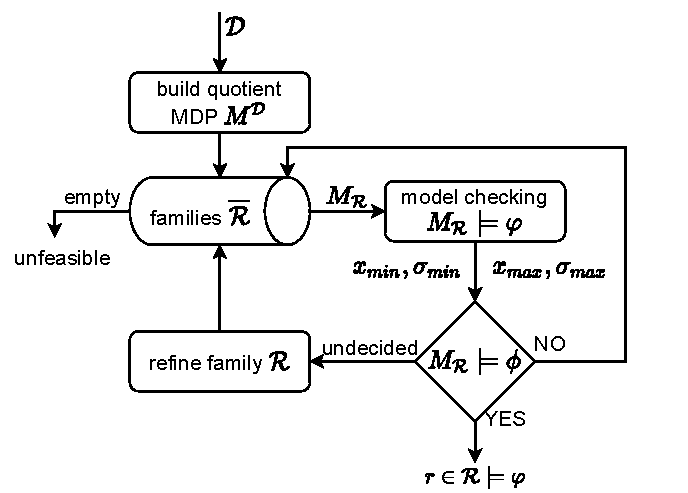
\includegraphics[width=0.70\textwidth]{figures/ar_loop.pdf}
\caption{An \textit{Abstraction Refinement} (AR) analysing loop.}%
\label{fig:architecture}%
\end{figure*}


In such a~case, we split the~undecidable family of Markov chains into two derived subfamilies. 
Then each of them represents the~input for deductive oracle,~which analyse them using the~technique introduced above.
When derived subfamilies are still undecidable, we refine them into smaller and smaller subfamilies until we find a~feasible solution or explore the~whole family.
When the~sub-family represents concrete realisation,~so it induces an~MC and not MDP ($x_{min} = x_{max}$),~such family is necessarily decided and have not split.
Moreover,~since the~family size is finite,~the~presented technique has guaranteed the~termination for these two reasons.
 
\paragraph{TODO NAME.} The~novel integrated approach,~the~so-called \textit{hybrid} method,~combines both these oracles and can thus take advantage of the~benefits offered by both approaches~\cite{roman-DP,tacas21}.
We illustrate the~cooperation between the~individual units within this method in Figure~\ref{fig:adaptivesynt}.
The~learner unit maintains the~subfamilies queue $\rlz' \subseteq \rlzf$ for subsequent processing and decides which oracle is selected based on their previous efficiency.
The~\textit{CE-Oracle} analyses the~family member $r$ and,~when it satisfies the~given specification $\varPhi$,~then returns it as a~solution.
On the~other hand,~it can generalise the~analysed realisation $r$ into a~subfamily $\rlz'$,~and the~learner unit can discard it from the~whole design space $\rlzf$.
Moreover,~this oracle exploits the~MDP bounds when constructing counterexamples,~thanks to which it can generate more petite generalisations.
The~\textit{Abstr-Oracle} analyses a~given sub-family $\rlz \subseteq \rlzf$,~and according to the~result,~it performs the~subsequent action.
When all realisations $r \in \rlz$ satisfy $\varPhi$,~then it returns the~overall synthesis result as feasible.
In another case,~when all realisations violate $\varPhi$,~the~whole analysed sub-family $\rlz$ will be discarded from the~families queue $\rlzf$ by the~learner.
The last option returns safe bounds on the best- and worst-case behaviour of all realisations in $\rlz$ considered $\varPhi$ when the analysis result is inconclusive.

\begin{figure}[ht!]
    \centering
     \begin{tikzpicture}
    \node[rectangle, draw, inner sep=8pt] (learner) {Learner};
    \node[rectangle, draw, inner sep=8pt,right=2.7cm of learner] (oracle) {CE-Oracle};
       \node[rectangle, draw, inner sep=8pt,left=2.7cm of learner] (abst) {Abstr-Oracle};
    \node[above=0.5cm of learner] (rlz) {$\rlzf$};
    \draw[->] (rlz) -- (learner);
    \node[above=0.5cm of oracle] (phi) {$\varPhi$};
    \draw[->] (phi) -- (oracle);
    \node[above=0.5cm of abst] (phiab) {$\varPhi$};
    \draw[->] (phiab) -- (abst);
    \draw[->] (learner) edge[bend left=10] node[above] {\scriptsize{$r \in \rlzf$}+bounds} (oracle);
    \draw[->] (oracle) edge[bend left=10] node[below] {\scriptsize{$\rlz' \subseteq \rlzf$ violate $\varPhi$}} (learner);
      \draw[->] (learner) edge[bend right=10] node[above] {\scriptsize{$\rlz \subseteq \rlzf$}} (abst);
    \draw[->] (abst) edge[bend right=10] node[below,align=center] {\scriptsize{bounds \emph{or} $\rlz$ violates}} (learner);
    
    \node[below=0.4cm of oracle] (sat) {$r \models \varPhi$};
    \draw[->] (oracle) -- (sat);
    \node[below=0.4cm of abst] (allsat) {each $r \in \rlz$, $r \models \varPhi$};
    \draw[->] (abst) -- (allsat);
    \node[below=0.4cm of learner] (unsat) {no $r \models \varPhi$};
    \draw[->] (learner) -- (unsat);
    \end{tikzpicture}
  \vspace{-0,5em}
    \caption{Oracle-guided synthesis (adapted from~\cite{tacas21}).}
    \label{fig:adaptivesynt}.
    \vspace{-1em}
\end{figure}

\paragraph{Hybrid Method.}
An~extended synthesis approach was introduced in~\cite{roman-DP,tacas21} using the~abstraction refinement to family prune and accelerating the~construction of counter-examples by CE-oracle.
Its main idea is to perform a~limited number of abstraction refinement loops and then invoke CEGIS to one of the~refined sub-families.
It turned out that a~moment of the~switching can be crucial,~and therefore,~the~method has to detect the~rightest moment.
One AR iteration is typically significantly slower than one CEGIS iteration since the~AR iteration involves an~MDP model-checking,~which inspires whole method workflow.
The~advance of the~hybrid methods is also constructing counter-examples within the~CEGIS loop,~where it uses a~fast greedy approach providing smaller generalisations.

\begin{algorithm}[H]
\hspace*{\algorithmicindent} \textbf{Input:} A MCs family $\fml$, a reachability property $\varphi$. \\
\hspace*{\algorithmicindent} \textbf{Output:} $Realization\; r \in \rlzf \; s.t. \; \mathcal{D}_r \models \varphi$, otherwise UNSAT. \\
\vspace*{-1.5em}
\begin{algorithmic}[1]
    \STATE $\rlzf \leftarrow \{ \rlz^{\fml} \}$ \hfill \textbf{// each analysed (sub)-family also holds bounds}
    \STATE $\delta_{CEGIS} \leftarrow 1$ \hfill \textbf{// time allocation factor for CEGIS}
    \WHILE{$\rlzf \neq \emptyset$}
        \STATE result, $\rlzf'$, $\sigma_{AR}$, $t_{AR}$ $\leftarrow$ AR($\rlzf$, $\varphi$)
        \IF{\textbf{satisfiable}(result)}
            \RETURN result
        \ELSE
            \STATE result, $\rlzf''$, $\sigma_{CEGIS}$ $\leftarrow$ CEGIS($\rlzf'$, $\varphi$)
            \IF{\textbf{satisfiable}(result)}
                \RETURN result
            \ELSE
                \STATE $\delta_{CEGIS}$ $\leftarrow$ $\sigma_{CEGIS}$ / $\sigma_{AR}$
                \STATE $\rlzf$ $\leftarrow$ $\rlzf''$
            \ENDIF
        \ENDIF
    \ENDWHILE
    \RETURN{UNSAT}
\end{algorithmic}
\caption{Hybrid method: Feasibility synthesis with single property.}
\label{alg:hybrid}
\end{algorithm}

As we said above,~this \textit{novel integrated} method combines inductive and deductive oracles,~and we briefly summarise their operation.
CEGIS iterates through all family members (realisations) until it reached the~satisfying realisation,~if such exists,~or when it explores the~whole design space.
Moreover,~it constructs counter-examples whenever the~analysed realisation $r \in \fmlr$ unsatisfying the~given specification $\varPhi$.
Realisations subset $\rlz' \subseteq \rlzf$ represents such counter-examples that CEGIS subsequently prunes from the~analysed design space $\rlzf$.
On the~other hand,~an AR loop builds MDP models from the~sub-families queue $\rlz \subseteq \rlzf$ that model-checkers analyse in follows.
When the~analysis results are inconclusive,~an AR refines the~analysed sub-family and  stores the~obtained satisfiability bounds for further processing within CEGIS loop.
Method allocates the~time per both loop according to their performance,~e.g.,~it can consider the~number of pruned MCs per timed unit and estimates an~efficiency from it.
Namely,~when it notices that AR prunes sub-families twice as slow as CEGIS,~it increases time twice in the~next round for CEGIS.
The resulting algorithm is summarised in Algorithm~\ref{alg:hybrid},~adapted from~\cite{tacas21}.